% Options for packages loaded elsewhere
\PassOptionsToPackage{unicode}{hyperref}
\PassOptionsToPackage{hyphens}{url}
\PassOptionsToPackage{dvipsnames,svgnames,x11names}{xcolor}
%
\documentclass[
]{agujournal2019}

\usepackage{amsmath,amssymb}
\usepackage{iftex}
\ifPDFTeX
  \usepackage[T1]{fontenc}
  \usepackage[utf8]{inputenc}
  \usepackage{textcomp} % provide euro and other symbols
\else % if luatex or xetex
  \usepackage{unicode-math}
  \defaultfontfeatures{Scale=MatchLowercase}
  \defaultfontfeatures[\rmfamily]{Ligatures=TeX,Scale=1}
\fi
\usepackage{lmodern}
\ifPDFTeX\else  
    % xetex/luatex font selection
\fi
% Use upquote if available, for straight quotes in verbatim environments
\IfFileExists{upquote.sty}{\usepackage{upquote}}{}
\IfFileExists{microtype.sty}{% use microtype if available
  \usepackage[]{microtype}
  \UseMicrotypeSet[protrusion]{basicmath} % disable protrusion for tt fonts
}{}
\makeatletter
\@ifundefined{KOMAClassName}{% if non-KOMA class
  \IfFileExists{parskip.sty}{%
    \usepackage{parskip}
  }{% else
    \setlength{\parindent}{0pt}
    \setlength{\parskip}{6pt plus 2pt minus 1pt}}
}{% if KOMA class
  \KOMAoptions{parskip=half}}
\makeatother
\usepackage{xcolor}
\setlength{\emergencystretch}{3em} % prevent overfull lines
\setcounter{secnumdepth}{5}
% Make \paragraph and \subparagraph free-standing
\ifx\paragraph\undefined\else
  \let\oldparagraph\paragraph
  \renewcommand{\paragraph}[1]{\oldparagraph{#1}\mbox{}}
\fi
\ifx\subparagraph\undefined\else
  \let\oldsubparagraph\subparagraph
  \renewcommand{\subparagraph}[1]{\oldsubparagraph{#1}\mbox{}}
\fi


\providecommand{\tightlist}{%
  \setlength{\itemsep}{0pt}\setlength{\parskip}{0pt}}\usepackage{longtable,booktabs,array}
\usepackage{calc} % for calculating minipage widths
% Correct order of tables after \paragraph or \subparagraph
\usepackage{etoolbox}
\makeatletter
\patchcmd\longtable{\par}{\if@noskipsec\mbox{}\fi\par}{}{}
\makeatother
% Allow footnotes in longtable head/foot
\IfFileExists{footnotehyper.sty}{\usepackage{footnotehyper}}{\usepackage{footnote}}
\makesavenoteenv{longtable}
\usepackage{graphicx}
\makeatletter
\def\maxwidth{\ifdim\Gin@nat@width>\linewidth\linewidth\else\Gin@nat@width\fi}
\def\maxheight{\ifdim\Gin@nat@height>\textheight\textheight\else\Gin@nat@height\fi}
\makeatother
% Scale images if necessary, so that they will not overflow the page
% margins by default, and it is still possible to overwrite the defaults
% using explicit options in \includegraphics[width, height, ...]{}
\setkeys{Gin}{width=\maxwidth,height=\maxheight,keepaspectratio}
% Set default figure placement to htbp
\makeatletter
\def\fps@figure{htbp}
\makeatother
\newlength{\cslhangindent}
\setlength{\cslhangindent}{1.5em}
\newlength{\csllabelwidth}
\setlength{\csllabelwidth}{3em}
\newlength{\cslentryspacingunit} % times entry-spacing
\setlength{\cslentryspacingunit}{\parskip}
\newenvironment{CSLReferences}[2] % #1 hanging-ident, #2 entry spacing
 {% don't indent paragraphs
  \setlength{\parindent}{0pt}
  % turn on hanging indent if param 1 is 1
  \ifodd #1
  \let\oldpar\par
  \def\par{\hangindent=\cslhangindent\oldpar}
  \fi
  % set entry spacing
  \setlength{\parskip}{#2\cslentryspacingunit}
 }%
 {}
\usepackage{calc}
\newcommand{\CSLBlock}[1]{#1\hfill\break}
\newcommand{\CSLLeftMargin}[1]{\parbox[t]{\csllabelwidth}{#1}}
\newcommand{\CSLRightInline}[1]{\parbox[t]{\linewidth - \csllabelwidth}{#1}\break}
\newcommand{\CSLIndent}[1]{\hspace{\cslhangindent}#1}

\usepackage{url} %this package should fix any errors with URLs in refs.
\usepackage{lineno}
\usepackage[inline]{trackchanges} %for better track changes. finalnew option will compile document with changes incorporated.
\usepackage{soul}
\linenumbers
\makeatletter
\makeatother
\makeatletter
\makeatother
\makeatletter
\@ifpackageloaded{caption}{}{\usepackage{caption}}
\AtBeginDocument{%
\ifdefined\contentsname
  \renewcommand*\contentsname{Table of contents}
\else
  \newcommand\contentsname{Table of contents}
\fi
\ifdefined\listfigurename
  \renewcommand*\listfigurename{List of Figures}
\else
  \newcommand\listfigurename{List of Figures}
\fi
\ifdefined\listtablename
  \renewcommand*\listtablename{List of Tables}
\else
  \newcommand\listtablename{List of Tables}
\fi
\ifdefined\figurename
  \renewcommand*\figurename{Figure}
\else
  \newcommand\figurename{Figure}
\fi
\ifdefined\tablename
  \renewcommand*\tablename{Table}
\else
  \newcommand\tablename{Table}
\fi
}
\@ifpackageloaded{float}{}{\usepackage{float}}
\floatstyle{ruled}
\@ifundefined{c@chapter}{\newfloat{codelisting}{h}{lop}}{\newfloat{codelisting}{h}{lop}[chapter]}
\floatname{codelisting}{Listing}
\newcommand*\listoflistings{\listof{codelisting}{List of Listings}}
\makeatother
\makeatletter
\@ifpackageloaded{caption}{}{\usepackage{caption}}
\@ifpackageloaded{subcaption}{}{\usepackage{subcaption}}
\makeatother
\makeatletter
\makeatother
\ifLuaTeX
  \usepackage{selnolig}  % disable illegal ligatures
\fi
\IfFileExists{bookmark.sty}{\usepackage{bookmark}}{\usepackage{hyperref}}
\IfFileExists{xurl.sty}{\usepackage{xurl}}{} % add URL line breaks if available
\urlstyle{same} % disable monospaced font for URLs
\hypersetup{
  pdftitle={Studentsourcing - aggregating and re-using data from a practical cell biology course},
  pdfauthor={Joachim Goedhart},
  pdfkeywords={Crowdsourcing, Data visualization, FAIR data, Dashboard},
  colorlinks=true,
  linkcolor={blue},
  filecolor={Maroon},
  citecolor={Blue},
  urlcolor={Blue},
  pdfcreator={LaTeX via pandoc}}


\draftfalse

\begin{document}
\title{Studentsourcing - aggregating and re-using data from a practical
cell biology course}

\authors{Joachim Goedhart\affil{1}}
\affiliation{1}{Molecular Cytology, SILS - University of Amsterdam, The
Netherlands, }
\correspondingauthor{Joachim Goedhart}{j.goedhart@uva.nl}


\begin{abstract}
Data that is generated by students during a course is often lost as
there is no central, structured storage of those data. The loss of data
prevents its re-use. To enable re-use of the data, I present an approach
to collect, aggregate and re-use data that is generated by students in a
practical course on cell biology. The course runs annually and I have
recorded the data that was generated by students over 3 years. Two
use-cases illustrate how this data can be aggregated and re-used either
for the scientific record or for teaching. As the data is obtained by
different students, in different groups, over different years, it is an
excellent opportunity to discuss experimental design and modern data
visualization methods such as the superplot. The first use-case shows
how central data storage provides a unique opportunity to get precise
quantitative data due to the large sample size. The second use-case
demonstrates how the data can be presented as an online, interactive
dashboard, providing real-time data of the measurements. Both use cases
illustrate how data can be effectively aggregated and re-used.
\end{abstract}

\section*{Plain Language Summary}
Data acquired by students has value and in this work we present ways to
collect and re-use that data.


\hypertarget{sec-introduction}{%
\section*{Introduction}\label{sec-introduction}}
\addcontentsline{toc}{section}{Introduction}

Teaching practical skills in a lab course is a crucial part of education
in biology, biomedical science, and life sciences. In these lab courses
data is generated, reported and interpreted, much like \emph{real}
experimental lab work. However, students use their data just for their
own lab report and the data is not centrally stored or aggregated. As a
consequence, most of the data that is gathered in a lab course is lost.
Yet, these data are potentially useful. Especially for larger course, an
impressive amount of data under well-controlled conditions can be
generated. Therefore, by collecting and aggregating the data of multiple
students over multiple years, one can easily gather a large dataset with
high numbers of independent observations, or as defined by Lazic et al.
(2018), biological replicates and experimental units.

Microscopy is an essential tool in cell biology. The use of microscopes
to observe cells and organisms has changed from a qualitative,
descriptive approach, into a quantitative method (Renz, 2013; Senft et
al., 2023; Wait et al., 2020; Waters, 2009). The development of digital
cameras and image analysis software has catalyzed this transition
(Carpenter, 2007). Therefore, experiments that use microscopes are often
followed by bioimage analysis to extract quantitative information from
the data. To teach these skills, we combine a basic course on microscopy
in a course on cell biology with teaching image processing and analysis
in ImageJ/FIJI (Schneider et al., 2012). In a typical year, over one
hundred students are enrolled in this course and therefore, a
substantial amount of data is generated in the course.

We decided to collect the data that was generated by the students in the
lab course over several years and store the measurement results in a
central location. The data by itself can be valuable for the scientific
community as precise estimates with good statistics can be obtained.
Moreover, the data are a starting point to discuss data visualization,
experimental design and how experimental design affects the statistics
and interpretation of data. Here, we report the methods to collect,
process and visualize the data and demonstrate some of the ways the data
can be re-used.

\hypertarget{sec-data-methods}{%
\section*{Methods}\label{sec-data-methods}}
\addcontentsline{toc}{section}{Methods}

For full reproducibility, this document is written using Quarto (Posit,
\url{https://quarto.org/}), and the source code of the manuscript and
the notebooks, and the data are availble in a repository:
\url{https://github.com/JoachimGoedhart/MS-StudentSourcing}

\hypertarget{use-case-1}{%
\subsection*{Use case 1}\label{use-case-1}}
\addcontentsline{toc}{subsection}{Use case 1}

\emph{Sample preparation and measurements}

HeLa cells are cultured according to standard procedures and seeded 1 or
2 days before the treatment on 12 mm diameter glass coverslips. HeLa
cells are incubated with 10 µM EdU for 30 minutes at 37 ˚C. The cells
are fixed with 4\% formaldehyde in PBS and permeabilised with 0.1\%
Triton X-100 in PBS. Click chemistry is performed with 9 µM Cy3-azide
and 2 mM CuSO\textsubscript{4}. To start the reaction, 20 mg/ml
ascorbate (final concentration) is added and the solution is used
immediately to stain the cells. After 30 minutes, the cells are washed
3x with PBS and the sample is incubated with 0.1 µg/ml DAPI for 5
minutes. Samples are mounted in Mowiol and used for observation with
fluorescence microscopy. Images of at least 100 cells are acquired with
the DAPI and TRITC filters sets. The nuclei in both channels are counted
by hand, or in an automated way by segmentation and `particle analysis'
in imageJ to calculate the percentage of cells that are positive for Cy3
fluorescence, reflecting cells in the S-phase.

\emph{Data collection}

The data of the measurements is collected on voluntary basis through a
Google Form, an example of which is shown in \emph{figure XX}. The data
that is recorded is the group (A/B/C/D), the percentage of cells in the
S-phase for two methods, i.e.~manual and using ImageJ/FIJI. The form is
easy to set up and the data is collected in Google Sheets, yielding four
columns; Timestamp, Group, and two columns with percentages of S-phase
determined by the two methods.

\emph{Data processing \& visualization}

The data that is in the Google Sheet can be downloaded and read into R
(R Core Team, 2022) as a CSV. All subsequent processing and data
visualization is done with \texttt{\{rmarkdown\}} (Allaire et al.,
2022). The R Markdown file and a rendered version as HTML are available
on Github: \url{https://github.com/JoachimGoedhart/PreciSeR}. The
cleaning of the data consists of removing empty cells, changing the
column names, conversion to a tidy format, forcing the data into a
`numeric' type and filtering for sensible values (anything outside the
generous range of 0-100 will be removed).

\hypertarget{use-case-2}{%
\subsection*{Use case 2}\label{use-case-2}}
\addcontentsline{toc}{subsection}{Use case 2}

\emph{Sample preparation and measurements}

A buccal swab is used to harvest cheek cells by scraping
\textasciitilde5 times over the inside of the cheek. The tip of the
sample collector is dipped into an eppendorf tube with 40 µl PBS, and
the cells are transferred to an object slide by touching the slide with
the tip. Next, 10 µl of 0.1\% methyleneblue solution is added and the
sample is enclosed by a square coverslip (22 x 22 mm). The sample is
used immediately to observe the cells with a Leica microscope, equipped
with a Lumenera camera. A 20x or 40x objective is used to observe and
image the cells. A separate image of a micrometer
(\href{https://www.fishersci.com/shop/products/stage-graticules-s8/5028481}{Electron
Microscopy Sciences 6804208, Stage Micrometer S8, Horizontal Scale, 1 mm
Length}) is acquired at the same magnification. The images are processed
in ImageJ/FIJI and the dimensions of the images are calibrated with the
micrometer image. The line tool is used to measure the diameter of the
cells (the longest axis).

\emph{Data collection}

The data of the measurements is collected through a Google Form, an
example of which is shown in \emph{figure XX}. The data that is recorded
by the form is the group (A/B/C/D), the size measurements of the cheek
cells and the size measurements of the nucleus. The data is aggregated
in a Google Sheet which has four columns with data on Timestamp, Group,
size of cells, size of nuclei. When correctly uploaded, the two columns
with the size data have comma separated values of 10 measurements.

\emph{Data processing}

The data that is in the Google Sheet can be downloaded and read into R
as a CSV. All subsequent processing and data visualisation and
presentation in dashboard style is done in R. The code is available on
Github: \url{https://github.com/JoachimGoedhart/CellSizeR}. The cleaning
of the data consist of removing empty cells, changing the column names,
listing all individual measurements in a single row, forcing the data
into a `numeric' type and filtering for sensible values (anything
outside the generous range of 0-1000 will be removed). A detailed
protocol that explains the processing is available as protocol 10
(Goedhart, 2022).

\emph{Data visualisation}

A dashboard is composed in R Markdown with the
\texttt{\{flexdashboard\}} package. The code is available here:
\url{https://github.com/JoachimGoedhart/CellSizeR} and the live
dashboard is available online:
\url{https://amsterdamstudygroup.shinyapps.io/CellSizeR/}

\hypertarget{sec-results}{%
\section*{Results}\label{sec-results}}
\addcontentsline{toc}{section}{Results}

\hypertarget{use-case-1-determination-of-the-percentage-of-cells-in-s-phase}{%
\subsection*{Use case 1: Determination of the percentage of cells in
S-phase}\label{use-case-1-determination-of-the-percentage-of-cells-in-s-phase}}
\addcontentsline{toc}{subsection}{Use case 1: Determination of the
percentage of cells in S-phase}

The aim of the experiment is is to determine the number of cells, as
percentage, that are in the S-phase. To this end, students stain cells
that are treated with EdU and they use these samples to quantify the
percentage of cells in the S-phase in two ways (manual and
semi-automated). The results are uploaded via a Google Form. The
collected data can be analysed in multiple ways and here we used it to
compare the two analysis methods and, secondly, to obtain an estimate
for the percentage of S-phase cells. The data on the two analysis
methods, manual and automated, is paired and can be visualised by a
doplot in which the pairs of the data are connected
(Figure~\ref{fig-paired-data}). The slopes of the lines vary a lot,
whereas the average values per year between the two methods is similar.
This implies that there can be substantial differences between the two
methods, with roughly a similar number of cases where the automated
analysis over- or underestimates the percentage, relative to the manual
analysis.

\begin{figure}[H]

{\centering 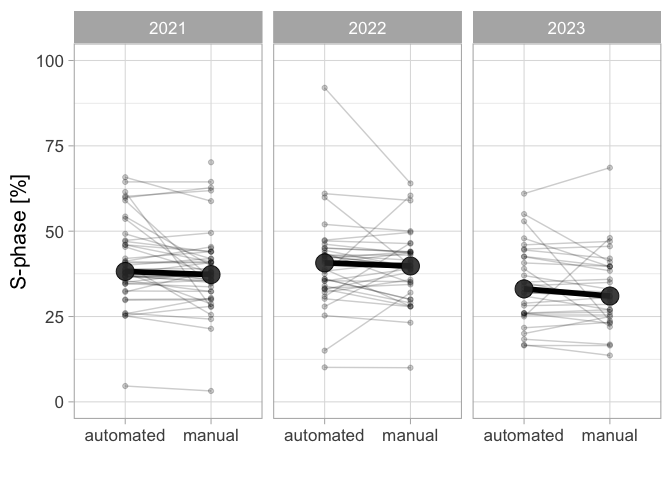
\includegraphics{index_files/figure-latex/fig-paired-data-output-1.png}

}

\caption{\label{fig-paired-data}Comparing the manual and automated
analysis. Source:
\href{https://JoachimGoedhart.github.io/MS-StudentSourcing/notebooks/PreciSe-preview.html\#cell-fig-paired-data}{The
percentage of cells in the S-phase}}

\end{figure}

There is increasing attention on effects of experimental design on data
analysis and visualization. The recently proposed superplot to
distinguish biological and technical replicates is an intuitive and
straightforward way to communicate the design (Lord et al., 2020). The
data on S-phase consists of both technical and biological replicates and
is therefore ideally suited to explain the importance of correctly
identifying the independent measurements. Here, we treat the data from
each group as biological replicate, and the measurements within each
group as a technical replicate. The reason is that a group of students
all stain cells that are from the same passage number and treated at the
same time and is therefore a technical replicate. On the other hand,
different groups stain different passages of cells and so we treat these
as independent observations. When the data is plotted for each
individual technical replicate (Figure~\ref{fig-superplot}), it can be
observed that we received multiple submissions per group, leading to a
precise measurement per group. The median values range from 23\% to
44\%. The average value of the independent observations is 36.7\%
{[}N=12, 95\%CI = 33.0\%-40.3\%{]}.

\begin{figure}[H]

{\centering 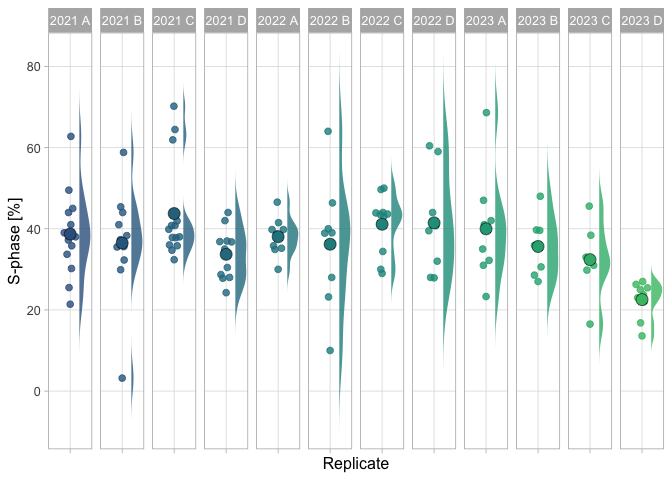
\includegraphics{index_files/figure-latex/fig-superplot-output-2.png}

}

\caption{\label{fig-superplot}Data on the percentage of cells in e
S-phase based on manual analysis. Each group \& year defines an
independent observations and is shown as dotplot and the distribution.
The larger dot reflects the median value. Source:
\href{https://JoachimGoedhart.github.io/MS-StudentSourcing/notebooks/PreciSe-preview.html\#cell-fig-superplot}{The
percentage of cells in the S-phase}}

\end{figure}

\hypertarget{use-case-2-comparing-new-results-with-historical-data}{%
\subsection*{Use case 2: Comparing new results with historical
data}\label{use-case-2-comparing-new-results-with-historical-data}}
\addcontentsline{toc}{subsection}{Use case 2: Comparing new results with
historical data}

The aim of the experiment is to determine the average size (diameter) of
a human cheek cell and nucleus. To this end, the students acquire images
of their own, stained cheek cells and measure the size of the cell and
its nucleus. At least 10 measurements are made and the data are uploaded
with a Google form. Each sample is an independent observation as it
originates from a unique human specimen. The main learning objective for
the students is to carry out the cell size measurements based on the
images that are acquired. One important aspect to get to the right
solution is the correct calibration of the field of view with a micro
ruler. When the calibration is done incorrectly, this will affect the
accuracy of the measurement, usually by an order of magnitude. To
evaluate their results, the students can compare their own data with the
historical data that is displayed on an online, interactive dashboard:
\url{https://amsterdamstudygroup.shinyapps.io/CellSizeR/}. On the
dashboard, users can select the data from all measurements, or from a
single year. A histogram visualizes the distribution of individual data
for both the cell and the nucleus and the bins of the histogram can be
adjusted. Since the sizes vary susbtantially, the data can be shown on a
log-scale as well (Figure~\ref{fig-histogram}). The dashboard shows the
same graph as depicted in Figure~\ref{fig-histogram}, but it is
interactive in the sense that by hovering over the plots, the exact
values of the data can be inferred as well. The dashboard also shows the
data for the 4 different groups and the size distribution of the cells
by violin plots.

\begin{figure}[H]

{\centering 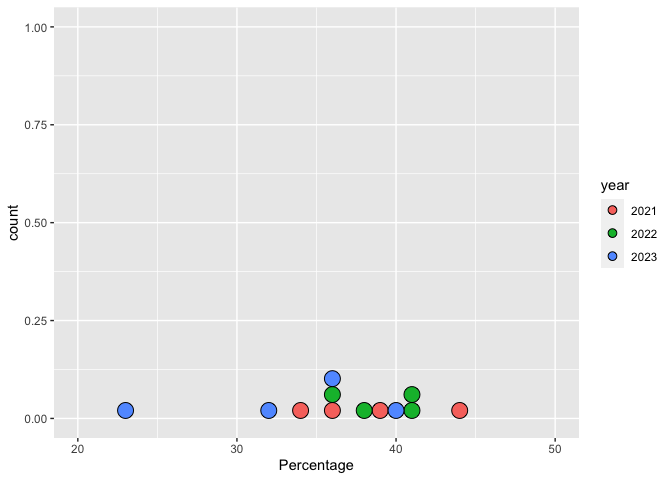
\includegraphics{index_files/figure-latex/fig-histogram-output-1.png}

}

\caption{\label{fig-histogram}Distribution of the measured size of human
cheek cells and their nucleus. Data from three years. Source:
\href{https://JoachimGoedhart.github.io/MS-StudentSourcing/notebooks/CellSizeR-preview.html\#cell-fig-histogram}{Summarizing
the size of cells}}

\end{figure}

The dashboard clearly shows a multimodal distribution of the results,
which is caused by a set of incorrect measurements due to incorrect
calibration. Still, if we assume that the majority of measurements is
correct, it is possible for the students to make a fair comparison and
discuss their results in the context of the historical data.

\hypertarget{sec-conclusion}{%
\section*{Conclusion}\label{sec-conclusion}}
\addcontentsline{toc}{section}{Conclusion}

Data that is generated in courses is often recorded by individual
students or groups of students in reports. However, it can be valuable
and interesting to collect and use these data. Here, I present a
flexible and open-source approach to collect and display data from a
large group of students and over several years. A combination of Google
Forms/Sheets for data collection and R for data processing and
visualization is used. In the first use case, a R Markdown template is
used to process and visualize the data. In the second use case, the data
is displayed in dashboard style. The code is available and can be used
as a starting point for the processing and visualization of other
datasets.

Collecting and reusing the data has a number of advantageous aspects.
First, a high number of measurements increases the precision of the
measurement and therefore allows us to obtain precise numbers. Second,
the historical data can be shared with the students and they can
interpret and discuss their results in light of the existing data.
Third, the obtained data serves as material that can be used to teach
data manipulation, statistics and data visualization which is a
fundamental aspect of science (Sailem et al., 2016). The use cases
described in this paper deal with these aspects.

The aggregation of the data inevitably leads to a discussion on
experimental design, as this is important to establish whether
measurements are independent or not. This aspect of experimental design
has received attention over the last years (Aarts et al., 2015; Eisner,
2021; Sikkel et al., 2017) and it is valuable to teach this aspect of
data analysis and visualization. Although I have not implemented this
yet, I think that having students participate in the data aggregation,
creates a very practical opportunity to teach experimental design and
the identification of biological units (Lazic et al., 2018).

In conclusion, I feel it is valuable to collect data from practical
courses and here we report one way to achieve that. I hope that serves
as a starting point for others that want to collect, store and use data
from large groups of students.

\hypertarget{acknowledgments}{%
\subsection*{Acknowledgments}\label{acknowledgments}}
\addcontentsline{toc}{subsection}{Acknowledgments}

A
\href{https://www.garrickadenbuie.com/blog/use-google-forms-and-r-to-track-data-easily/}{blog
post by Garrick Aden-Buie} was very helpful in the initial phase of this
project. Many thanks to the people involved in Quarto, which was used to
write and shape this paper. Most importantly, I'd like to thank all
students involved in the course that have generously shared their data,
making this a successful project.

\hypertarget{references}{%
\section*{References}\label{references}}
\addcontentsline{toc}{section}{References}

\hypertarget{refs}{}
\begin{CSLReferences}{1}{0}
\vspace{1em}

\leavevmode\vadjust pre{\hypertarget{ref-Aarts2015}{}}%
Aarts, E., Dolan, C. V., Verhage, M., \& Sluis, S. van der. (2015).
Multilevel analysis quantifies variation in the experimental effect
while optimizing power and preventing false positives. \emph{BMC
Neuroscience}, \emph{16}(1).
\url{https://doi.org/10.1186/s12868-015-0228-5}

\leavevmode\vadjust pre{\hypertarget{ref-RMarkdown}{}}%
Allaire, J., Xie, Y., McPherson, J., Luraschi, J., Ushey, K., Atkins,
A., et al. (2022). \emph{Rmarkdown: Dynamic documents for r}. Retrieved
from \url{https://github.com/rstudio/rmarkdown}

\leavevmode\vadjust pre{\hypertarget{ref-carpenter2007}{}}%
Carpenter, A. E. (2007). Software opens the door to quantitative
imaging. \emph{Nature Methods}, \emph{4}(2), 120--121.
\url{https://doi.org/10.1038/nmeth0207-120}

\leavevmode\vadjust pre{\hypertarget{ref-eisner2021}{}}%
Eisner, D. A. (2021). Pseudoreplication in physiology: More means less.
\emph{Journal of General Physiology}, \emph{153}(2).
\url{https://doi.org/10.1085/jgp.202012826}

\leavevmode\vadjust pre{\hypertarget{ref-goedhart2022}{}}%
Goedhart, J. (2022). \emph{DataViz protocols - an introduction to data
visualization protocols for wet lab scientists}. Zenodo.
\url{https://doi.org/10.5281/ZENODO.7257808}

\leavevmode\vadjust pre{\hypertarget{ref-lazic2018}{}}%
Lazic, S. E., Clarke-Williams, C. J., \& Munafò, M. R. (2018). What
exactly is {`}N{'} in cell culture and animal experiments? \emph{PLOS
Biology}, \emph{16}(4), e2005282.
\url{https://doi.org/10.1371/journal.pbio.2005282}

\leavevmode\vadjust pre{\hypertarget{ref-lord2020}{}}%
Lord, S. J., Velle, K. B., Mullins, R. D., \& Fritz-Laylin, L. K.
(2020). SuperPlots: Communicating reproducibility and variability in
cell biology. \emph{Journal of Cell Biology}, \emph{219}(6).
\url{https://doi.org/10.1083/jcb.202001064}

\leavevmode\vadjust pre{\hypertarget{ref-RCore}{}}%
R Core Team. (2022). \emph{R: A language and environment for statistical
computing}. Vienna, Austria: R Foundation for Statistical Computing.
Retrieved from \url{https://www.R-project.org/}

\leavevmode\vadjust pre{\hypertarget{ref-renz2013}{}}%
Renz, M. (2013). Fluorescence microscopy-A historical and technical
perspective. \emph{Cytometry Part A}, \emph{83}(9), 767--779.
\url{https://doi.org/10.1002/cyto.a.22295}

\leavevmode\vadjust pre{\hypertarget{ref-sailem2016}{}}%
Sailem, H. Z., Cooper, S., \& Bakal, C. (2016). Visualizing quantitative
microscopy data: History and challenges. \emph{Critical Reviews in
Biochemistry and Molecular Biology}, \emph{51}(2), 96--101.
\url{https://doi.org/10.3109/10409238.2016.1146222}

\leavevmode\vadjust pre{\hypertarget{ref-schneider2012}{}}%
Schneider, C. A., Rasband, W. S., \& Eliceiri, K. W. (2012). NIH Image
to ImageJ: 25 years of image analysis. \emph{Nature Methods},
\emph{9}(7), 671--675. \url{https://doi.org/10.1038/nmeth.2089}

\leavevmode\vadjust pre{\hypertarget{ref-senft2023}{}}%
Senft, R. A., Diaz-Rohrer, B., Colarusso, P., Swift, L., Jamali, N.,
Jambor, H., et al. (2023). A biologist{'}s guide to planning and
performing quantitative bioimaging experiments. \emph{PLOS Biology},
\emph{21}(6), e3002167.
\url{https://doi.org/10.1371/journal.pbio.3002167}

\leavevmode\vadjust pre{\hypertarget{ref-sikkel2017}{}}%
Sikkel, M. B., Francis, D. P., Howard, J., Gordon, F., Rowlands, C.,
Peters, N. S., et al. (2017). Hierarchical statistical techniques are
necessary to draw reliable conclusions from analysis of isolated
cardiomyocyte studies. \emph{Cardiovascular Research}, \emph{113}(14),
1743--1752. \url{https://doi.org/10.1093/cvr/cvx151}

\leavevmode\vadjust pre{\hypertarget{ref-wait2020}{}}%
Wait, E. C., Reiche, M. A., \& Chew, T.-L. (2020). Hypothesis-driven
quantitative fluorescence microscopy {\textendash} the importance of
reverse-thinking in experimental design. \emph{Journal of Cell Science},
\emph{133}(21). \url{https://doi.org/10.1242/jcs.250027}

\leavevmode\vadjust pre{\hypertarget{ref-waters2009}{}}%
Waters, J. C. (2009). Accuracy and precision in quantitative
fluorescence microscopy. \emph{Journal of Cell Biology}, \emph{185}(7),
1135--1148. \url{https://doi.org/10.1083/jcb.200903097}

\end{CSLReferences}



\end{document}
